% Chapter 3 - Network perspective

\section{Introduction}

The previous chapter described how absorptive capacity has evolved over time. It also explained how the advent of open innovation helped ground the concept and highlighted the critical role of tacit knowledge in building absorptive capacity. Since a firm's absorptive capacity is partly determined by its ability to establish and maintain productive inter-organisational networks \citep{inkpen2005social}, the previous chapter with a suggestion to use social network analysis to assess practices that build absorptive capacity in open innovation. \medskip

This chapter introduces the reader to social networks, explains how these can facilitate innovation, and describes relevant socio-psychological theories pertaining to social network analysis. \medskip

\section{Social networks}

Networks provide a way of thinking about social systems, one that focuses on the relationships among entities that make up the system \citep{borgatti2013analyzing,robins2015doing}. One can represent networks mathematically as graphs consisting of a set of vertices and a set of edges that connect vertices \citep{newman2010networks}. Vertices represent actors or nodes in a social network. Actors can be individuals, groups, organisations, regions, nations, or even a bloc of countries. These may be distinguished by binary, categorical or continuous attributes. For example, consider an individual actor classified as female (binary attribute), who works for a particular organisation (categorical attribute), with a specific number of years work experience (continuous attribute). Edges represent relations or social ties between actors. Ties can be measured as directed or undirected and as binary or valued. Deciding whether to measure a tie as directed or undirected depends on the theoretical nature of the tie. For instance, co-membership is inherently undirected whereas authority is essentially directed. Directed and undirected ties can be measured as binary ties that either exist or do not exist, or as valued ties that can be stronger or weaker, transmit more or fewer resources, or have more or less frequent contact \citep{scott2011sage}.\medskip

Different types of relations may exist between actors with each type of relation giving rise to a corresponding network \citep{borgatti2013analyzing}. Measuring knowledge sharing ties would, for example, generate a knowledge sharing network. Assigning an attribute to the knowledge sharing tie allows us to qualify the relationship in terms of the content or frequency of knowledge sharing. Ties can be classified according to similarities between actors or by relational roles, relational cognition, and events \citep{borgatti2013analyzing}. Ties between actors who share something in common (e.g. spatial location, affiliated to the same body, participate in the same event, or share a common attribute) are referred to as similarity ties. Relational roles include kinship and other ties, such as friendship, advice, and managerial ties. Relational cognition refers to ties that are affective (e.g. like or dislike another actor) or perceptual (e.g. belief about the other actor) in nature. Relational events refer to ties defined by specific social interactions (e.g. a transaction of some kind) and flows (e.g. knowledge flows).\medskip

Some ties are dependent on others. An example is friendship, which usually develops because of an pre-existing similarity tie (e.g. both actors live in the same neighbourhood, attend the same school, or work at the same place) or via a relational event tie (e.g. actors were introduced to each other at a specific event or worked together on a particular project). Actors are more likely to share  knowledge (relational event) with others who have common interests (similarity tie) or with others they trust (relational cognition). \medskip 

\section{Socio-psychological theories}






\section{Social network analysis}

The aim of social network analysis is detecting and interpreting patterns of social ties between actors \citep{de2011exploratory}. Most basic questions in social network analysis involve the measurement and modelling of particular structural properties \citep{butts2008social}. To fully understand the implications of social relations between actors, one has to consider how these are shaped by broader patterns of social interaction \citep{scott2011sage}. This requires more than simply measuring the basic characteristics of networks. A set of assumptions is needed to best describe and explain social phenomena of interest.  One may apply an existing socio-psychological theory to test hypotheses about social relations. Alternatively, one may use networks to explain specific outcomes or assess how social processes are influenced by network effects \citep{scott2011sage,borgatti2013analyzing}. \medskip\medskip



%monge and contractor

\subsection{Basic network descriptives}

Basic network descriptives Networks need to be described as directed or undirected. 

\subsection{Dyad and triad census}

\subsection{Degree distributions}

\subsubsection{Node centrality} 

\subsection{Structural holes}


\subsection{Connectivity}

\subsection{Network closure}

A frequent objective of social network analysis is the characterization of the properties of indi- vidual positions. We may seek to identify, for instance, persons in positions of prominence, or whose positions facilitate actions such as information dissemination. Alternately, we may also be interested in the social environment faced by a given individual, measuring features such as the extent to which his or her local environment is socially cohesive, or the diversity of his or her personal contacts. Such properties are generally summarized by means of node-level indices,

\subsubsection{Graph-level indices} 

While node-level indices describe structure which is local to a particular vertex, GLI quantify structural properties of the network as a whole.

%monge and contractor

\subsection{Conditional uniform graph models}



\subsection{Exponential random graph models}

Exponential random graph models are a class of statistical model for social networks originally developed by \citet{frank1986markov} and refined by \citet{wasserman1996logit} and \citet{pattison1999logit}. Exponential random graph models have the capacity to address complex social structures. Recent model derivations are able to examine both individual-level variables and structural relations simultaneously \citep{robins2007recent}. An exponential random graph model is essentially a pattern recognition device which breaks a network down into its constituent network motifs or configurations and then test if particular configurations occur more or less frequently than would be expected by chance alone. \medskip

Network configurations are patterns of social network ties assumed to represent underlying social processes or mechanisms \citep{lusher2014cooperative}. Exponential random graph models permit differentiation between structural network effects and processes related to actor attributes. Purely structural effects reflect endogenous processes in which ties form due to the presence or absence of other ties. Ties may also form due to actor attributes and are known as actor-relation effects. Exponential random graph models are particularly well-suited to this study, which is concerned about the individual, dyadic and organisational antecedents of absorptive capacity in open innovation networks.


\subsection{Mixed method social network analysis}

\section{Networked innovation}

\citet{granovetter1973strength} contends weak ties provide actors better access to new information and opportunities. Strong ties inhibit the flow of information from diverse distant sources. Sparse networks with an abundance of structural holes will allow strategically placed individuals to access diverse information and increase innovation output \citep{burt2004structural}. Networks with fewer structural holes promote trust generation and reduce opportunism, leading to more productive collaboration from the perspective of resource sharing \citep{ahuja2000collaboration}. \citet{burt2001structural} believes brokerage across structural holes in the disconnected network is the source of value, but closure is critical to realising the value buried in structural holes. Strong ties are more effective than weak ties in enhancing knowledge transfer and learning as well as an individual’s ability to benefit from collaborating with diverse partners \citep{rost2011strength,phelps2012knowledge}. Clarifying the implications of closed versus disconnected network structures for various organisational outcomes is important to our understanding of network resources \citep{ahuja2000collaboration}. \medskip

Individuals who are both strong knowledge producers and great collaborators enhance their firm’s innovative output \citep{grigoriou2014structural}. Relational stars provide firm-level knowledge advantages not only through their own superior recombinant efforts, but also through their capacity to make others around them more effective at knowledge recombination. Relational stars possess strong combination of both human and social capital, that is, a strong individual-level productivity performance combined with a highly consequential network position \citep{grigoriou2014structural}. \medskip
 
Diversity of knowledge and perspectives provided by bridging ties does not automatically translate into the generation of innovations \citep{ahuja2000collaboration}. Quality of relationships, and how these are managed, affects the ability of an individual to network strategically and expose them to opportunities \citep{uzzi1997social}. \citet{tortoriello2010activating} investigate the paradox in which diversity of knowledge and information available across organisational boundaries is necessary to spur innovation, yet at the same time may be a barrier for successful knowledge sharing and integration. Advantages stemming from bridging ties are contingent upon the configuration or microstructure of the ties forming the bridge \citep{tortoriello2010activating,tortoriello2015social}. Common third-party ties facilitate shared understanding, reduce friction due to differences in understanding, and promote cooperation and coordinated actions that are necessary to integrate and take advantage of diverse sources of knowledge (Tortoriello and Krackhardt 2010). Such brokerage is a crucial means by which intra- and inter-organisational networks evolve, expand and drive change (Obstfeld et al. 2014). The relationship between external knowledge and an individual’s ability to generate innovations is contingent on the type of knowledge and the individual’s position in the internal knowledge-sharing network (Tortoriello 2014; Tortoriello 2006). 

There is mounting evidence suggesting that network centrality predicts knowledge sharing in positive ways \citep[e.g.][]{freeman1979centrality,burt1992structural,tsai2001knowledge}. Every tie in an employee’s network represents a channel through which knowledge may flow to and from that employee \citep{anderson2008social}. Employees occupying central network positions have more relationships to draw on for the purpose of knowledge sharing. As a consequence of their extensive knowledge-sharing activity, employees in central network positions are likely to accumulate work-related knowledge, which positively affects not only their performance, but also their future knowledge sharing with colleagues \citep{sparrowe2001social}.

\section{Socio-psychological framework}

The flow of knowledge across firm boundaries is strongly influenced by individual attitudes, organisational cultures, and internal knowledge management processes. This chapter explains psychosocial theories considered important to this study. These include the theory of planned behaviour, self-determination theory, social identity theory, and social cognition theory. The aim is present the reader with an integrated theoretical framework for assessing knowledge sharing behaviour.

\subsection{Psychological theories}

\subsubsection{Trait theory}

Trait theory is an approach to the study of human personality. Traits define habitual patterns of behaviour, thought, and emotion. They differ across individuals and are stable over time. The \enquote{five-factor model} describes human personality in terms of five traits, namely \enquote{openness to experience}, \enquote{conscientiousness}, \enquote{extraversion}, \enquote{agreeableness}, and \enquote{neuroticism} \citep{mccrae1992introduction}. Table \ref{personality} lists key features of each trait. A person's personality can be described in terms of the combined strength of each trait. \medskip 

\begin{landscape}
	\begin{table}[]
		\centering
		\caption{Five-factor model personality traits \citep{mccrae1992introduction,howard1995big}.}
		\label{personality}
		\begin{tabular}{@{}lll@{}}
			\toprule
			Factor & Adjectives & Description \\ \midrule
			Extraversion (E) & \begin{tabular}[c]{@{}l@{}}Active\\ Assertive\\ Energetic\\ Enthusiastic\\ Outgoing\\ Talkative\end{tabular} & Extraversion refers to the number of relationships with which one is comforatble. High extraversion is characterised by a larger number of relationships and a larger proportion of one's time spent in enjoying them. Low extraversion is characterised by a smaller number of relationships and a smaller proportion of one's time spent in pursuing those relationships. \\
			Agreeableness (A) & \begin{tabular}[c]{@{}l@{}}Appreciative\\ Forgiving\\ Generous\\ Kind\\ Sympathetic\\ Trusting\end{tabular} & Agreeableness refers to the number of sources from which one takes one's norms for right behaviour. High agreeableness describes a person who defers to a great many norm sources, such as a spouse, religious leader, friend, boss, or popular culture idol. Low agreeableness describes one who is inclined to only follows one's inner voice. A highly agreeable person will march to the drumbeat of many different drummers, while a less agreeable person marches only to their own drumbeat. \\
			Conscientiousness (C) & \begin{tabular}[c]{@{}l@{}}Capable\\ Organised\\ Resourceful\\ Reliable\\ Responsible\\ Thorough\end{tabular} & Conscientiousness refers to the number of goals on which one is focused. High conscientiousness refers to a person who focuses on fewer goals and exhibits self-discipline associated with such focus. Low conscientiousness refers to one who pursues a larger number of goals and exhibits distractability and spontaneity associated with diffuse focus. \\
			Neuroticism (N) & \begin{tabular}[c]{@{}l@{}}Anxious\\ Self-pitying\\ Tense\\ Touchy\\ Worrying\end{tabular} & Neuroticism is a measure of affect and emotional control. Low levels of neuroticism indicate emotional stability whereas high levels of neuroticism increase the likelihood of experiencing negative emotions. A person with a high level of neuroticism is reactive and more easily bothered by stimuli in their environment. Such a person is prone to becoming unstable,worried, temperamental, and sad. A resistant person, on the other hand, needs strong stimuli to be provoked. \\
			Openness to experience & \begin{tabular}[c]{@{}l@{}}Artistic\\ Curious\\ Imaginative\\ Insightful\\ Original\\ Wide interests\end{tabular} & Openness refers the number of interests to which one is attracted and the depth to which those interests are pursued. High openness refers to a person with relatively more interests and, consequently, relatively less depth within each interest, while low openness refers to a person with relatively few interests and relatively more depth in each of those interests. \\ \bottomrule
		\end{tabular}
	\end{table}
\end{landscape}

Personality has been identified as a factor in knowledge sharing. \citet{matzler2008personality} found agreeableness, conscientiousness and openness to experience are positively correlated with knowledge sharing. People who are conscientious and introverted are more likely to share their tacit knowledge \citep{borges2012tacit}. \citet{stock2014impacts} found those who score higher on openness to experience are more likely to generate new ideas and that being introvert is positively associated with the successful realisation of ideas. They also found those who possess high levels of conscientiousness and neuroticism are more likely to commercially diffuse their innovations. \medskip

% why choose openness? cabrera2006determinants

\subsubsection{Self-determination theory}

Self-determination theory asserts humans are innately driven to seek out competence, autonomy and relatedness \citep{ryan2000self}. Central to self-determination theory is the distinction between controlled and autonomous motivation. Autonomy involves acting with a sense of volition and having the experience of choice. Being controlled involves acting under some sense of pressure \citep{gagne2005self}. Intrinsically motivated behaviour, driven by people’s interest in the activity itself, is essentially autonomous. Less interesting activities require extrinsic motivation, where people's actions depend on the perceived contingency between behaviour and desire for implicit approval or tangible rewards. Extrinsic motivation can vary in the degree to which it is autonomous versus controlled. Externally regulated behaviour is a prototype of controlled motivation. Other types of extrinsic motivation result when behavioural regulation and the value associated with it are internalised. Regulation that has been taken in by a person but not accepted as their own is said to be introjected. Such regulation may be seen as a relatively controlled form of internalised extrinsic motivation. With identified regulation, people feel a greater sense of autonomy because their behaviour is aligned to their personal goals and identities \citep{gagne2005self}. 

The primary difference between self-determination theory and other work motivation theories is that self-determination theory focuses on the relative strength of autonomous versus controlled motivation rather than on the total amount of motivation. Research shows that autonomous motivation facilitates effective performance and well-being, whereas controlled motivation can detract from those outcomes, particularly if the task requires creativity, cognitive flexibility, or deep processing of information \citep{gagne2005self}. This is particularly salient for innovation.


\subsection{Theory of planned behaviour}

The theory of planned behaviour suggests that actions and behaviours reliably follow intentions \citep{ajzen1985intentions}. Intentions capture the motivational factors that influence a behaviour e.g. how hard people are willing to try or make an effort to perform the behaviour. People’s behaviour is strongly influenced by their confidence in their ability to perform it (notions of perceived behavioural control or self-efficacy). The theory of planned behaviour postulates three conceptually independent determinants of intention. The first is the attitude toward the behaviour and refers to the degree to which a person has a favourable or unfavourable assessment of the behaviour in question. The second predictor is a social factor termed subjective norm, which refers to the perceived social pressure to perform or not to perform the behaviour. The third antecedent of intention is the degree of perceived behavioural control or self-efficacy which refers to how people rate the ease or difficulty of performing the behaviour, based on past experience as well as anticipated impediments and obstacles \citep{ajzen1991theory}.

The relative importance of attitude, subjective norm, and perceived behavioural control in the prediction of intention is expected to vary across behaviours and situations. Generally the more favourable the attitude and subjective norm with respect to a behaviour, the greater the perceived behavioural control, the stronger should be an individual’s intention to perform the behaviour under consideration \citep{ajzen1991theory}. 

Behaviour is a function of core beliefs relevant to the behaviour. These include behavioural beliefs which influence attitudes toward the behaviour, normative beliefs which constitute the underlying determinants of subjective norms, and control beliefs which provide the basis for perceptions of behavioural control \citep{ajzen1991theory} 

Behavioural intention can find expression in behaviour only if the behaviour in question is under volitional control \citep{ajzen1991theory}. 

Attitudes toward the behaviour, subjective norms with respect to the behaviour, and perceived control over the behaviour are usually found to predict behavioural intentions with a high degree of accuracy. In turn, these intentions, in combination with perceived behavioural control, can account for a considerable proportion of variance in behaviour \citep{ajzen1991theory}.


Motivation is a theoretical construct used to explain individual behaviour. A motive is what prompts a person to act in a certain way, or at least develop an inclination for specific behaviour. \citet{deci1985general} distinguish between intrinsic motivation, which refers to doing something because it is inherently interesting or enjoyable, and extrinsic motivation, which refers to doing something because it leads to a separable outcome. 

\citet{davenport1997ten} argues people need to be highly motivated to share knowledge with others. Past studies have looked at how firms can motivate people to share knowledge \citep[e.g.][]{cabrera2002knowledge,ipe2003knowledge,cabrera2006determinants,wang2010knowledge,witherspoon2013antecedents,von2015s}. \citet{ipe2003knowledge} refers to internal and external factors that influence the motivation to share knowledge. Internal factors include the perceived power attached to the knowledge and reciprocity that results from sharing. External factors include the relationship with the recipient and rewards for sharing \citep{ipe2003knowledge}. \medskip

There is a limit to what firms can do to motivate employees to share knowledge. \citet{davenport1997information} argue knowledge sharing is mostly a voluntary act, implying it is intrinsically motivated. \citet{bock2001breaking} find attitude toward knowledge sharing is negatively related to the expected rewards. In other words, incentives do not seem to alter the attitude that underlies knowledge sharing behaviour. One of the tenets of self-determination theory is that people are primarily motivated by innate needs for competence, autonomy, and relatedness \citep{ryan2000intrinsic}. People who share knowledge will perceive it as intrinsically satisfying because it is self-determined and allows them to increase their competencies \citep{kaser2001knowledge,gagne2005self,lam2010knowledge}. \medskip 

\citet{gagne2009model} describes a process model of knowledge-sharing motivation based on the combination of self-determination theory \citep{deci1985general,ryan2000self} and the theory of planned behaviour \citep{ajzen1991theory}. The model assumes knowledge sharing is intentional. The theory of planned behaviour contends intentions capture the motivational factors that influence a behaviour. Three factors influence intentions, namely attitude toward the behaviour, social norms regarding the behaviour, and beliefs about one’s control over the behaviour \citep{ajzen1991theory}.



research shows au- tonomous motivation leads to more positive behavioral out- comes than controlled motiva- tion

\medskip

Studies indicate knowledge sharing is mediated by intrinsic motivation \citep{bock2001breaking}. \citet{kaser2001knowledge} argue that as long as knowledge sharing is voluntary, sharing parties tend to perceive it as intrinsically satisfied because it is self-determined and allows them to increase their competencies. Intrinsic motivation is a key determinant of tacit knowledge transfer \citep{kaser2001knowledge,lam2010knowledge,dumbach2014establishing}. 

\subsubsection{Self-efficacy}

People with higher levels of self-efficacy are more likely to share knowledge and generate ideas with others \citep{tierney2002creative,lin2007effects}. 


\subsection{Social theories}

\subsubsection{Social exchange theory}

Social exchange theory views exchange as a social behaviour that may result in both economic and social returns \citep{lambe2001social}. Such behaviour emerges as a result of the social process of mutual reinforcement over time. Inadequate reinforcement or asymmetry in economic or social returns may result in the breakdown of social relations \citep{homans1961social}. Social behaviour may also emerge when people act to maximise the potential benefit of economic and social returns, where one person does another a favour, and while there is a general expectation of some future return, the exact nature of this return is not stipulated in advance \citep{blau1986exchange}. This can lead to differentiation in social status and power based on the dependence of some actors on others for valued goods and services \citep{emerson1962power}. Relative differences in power may result in an unequal distribution of returns across positions in a network of exchange. Tensions generated by power inequality can result in network extension where power-disadvantaged actors, rather than banding together to form coalitions to balance power, may alternatively seek out new relations, reducing their dependence on a given actor for valued resources \citep{cook2013social}. 

Trust is more likely to develop between partners when exchange occurs without explicit negotiations or binding agreements. Under such conditions, the risk and uncertainty of exchange provide the opportunity for partners to demonstrate their trustworthiness. Reciprocal exchange produces stronger trust and affective commitment than negotiated exchange \citep{molm2000risk}. 

Commitment is defined as an interpersonal attachment leading people to exchange repeatedly with the same partners. Research suggests that power-use and commitment are inversely related \citep{cook1978power}

%In this work we develop the perceived value of knowledge sharing as a multidimensional construct, grounded in assumptions of social exchange theory, consumer research and knowledge sharing literature. This conceptualization is intended to serve as a basis for the operationalization of perceived knowledge value in a future study on knowledge sharing intentions \citep{von2015s}.

\subsubsection{Social cognitive theory}

\subsubsection{Brokerage}

Brokerage underpins a broad range of organisational phenomena and represents an important mechanism by which intra- and inter-organisational networks evolve and drive change. It may be conceptualised as a social process that shapes interaction between two or more parties in a wide variety of triadic structures \citep{obstfeld2002knowledge}. Much of the organisational literature dealing with social structures considers brokerage in terms of an open triad, one in which a broker has ties to two alters who are not tied to one another. For example, \citet{marsden1982brokerage} defines brokerage as a mechanism \enquote{by which intermediary actors facilitate transactions between other actors lacking access or trust in one another}. \citet{fernandez1994dilemma} describe brokerage as a \enquote{relation in which one actor mediates the flow of resources or information between two other actors who are not directly linked}. They argue brokerage \enquote{does not permit the endpoints of a brokerage relation to be directly connected}. \citet{burt1992structural} believes brokers who stand between unconnected alters not only benefit from the novel information that such a structure affords, but are also able to play the disconnected actors against one another. This implies brokerage is more about empowerment of self than about empowering others. \medskip

\citet{gould1989structures} define a brokerage role as the position of j in an (i,j),(j,k) two-path with no (i,k) edge i.e. an intransitive triple. Adding a (k,i) edge to the representing cyclic closure does not undermine j's brokerage role. Brokerage involving transitive closure is not really brokerage in a cross-sectional context (Butts, personal communication).


\begin{table}[]
	\small
	\centering
	\caption{Gould-Fernandez brokerage roles}
	\label{gf_params}
	\begin{tabular}{@{}lcl@{}}
		\toprule
		\multicolumn{1}{c}{Role} & \multicolumn{1}{c}{Graphic} & \multicolumn{1}{c}{Explanation} \\ \midrule
		b\textsubscript{O} (liaison role)			&  \begin{minipage}{.2\textwidth} \centering 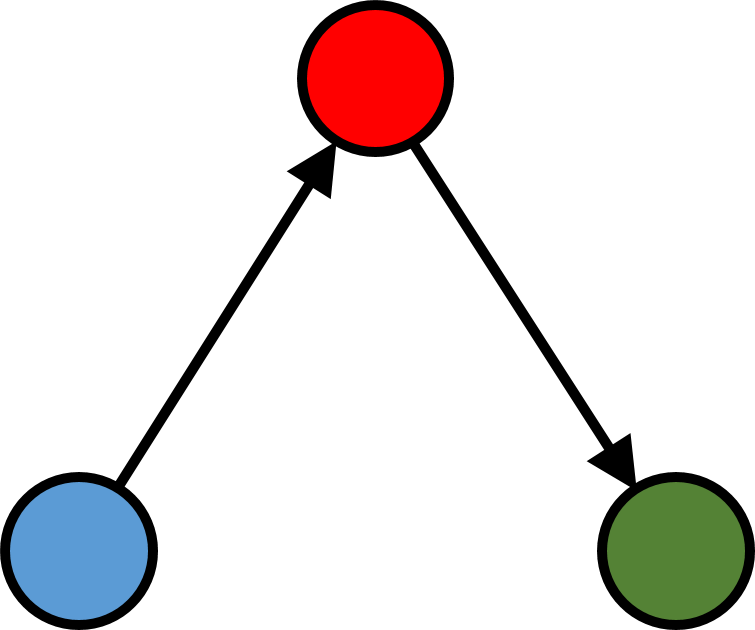
\includegraphics[width=0.4\linewidth]{Images/b_O} \end{minipage}	& \begin{tabular}[c]{l}Broker mediates contact between two\\ individuals from different groups,\\ neither of which is the group to\\ which he or she belongs.\end{tabular}\\ [10ex]
		b\textsubscript{IO} (representative role)	& \begin{minipage}{.2\textwidth} \centering 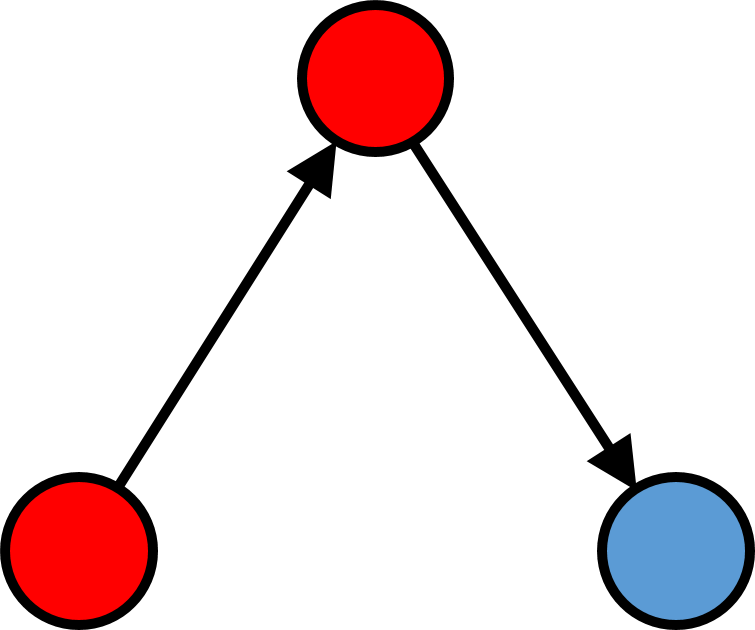
\includegraphics[width=0.4\linewidth]{Images/b_IO} \end{minipage}   & \begin{tabular}[c]{l}Broker mediates an outgoing contact\\ from an in-group member to an\\ out-group member.\end{tabular}\\ [10ex]
		b\textsubscript{OI} (gatekeeper role)		& \begin{minipage}{.2\textwidth} \centering 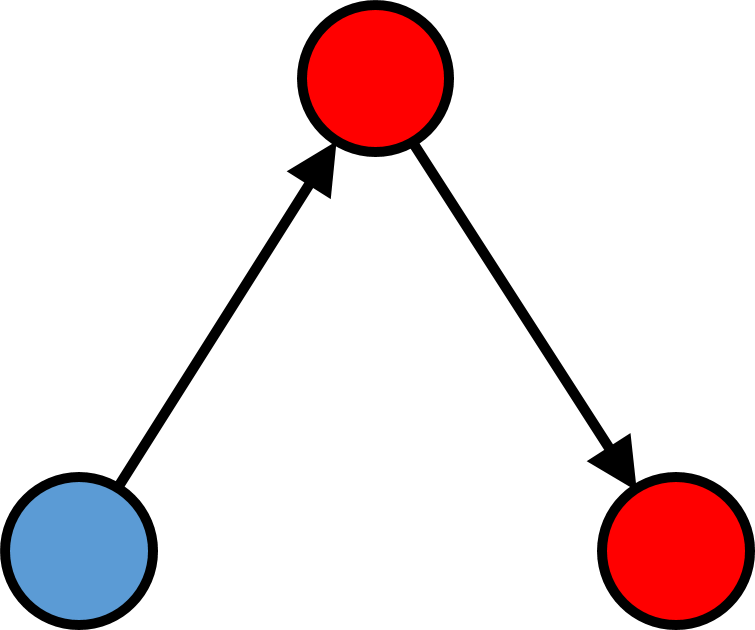
\includegraphics[width=0.4\linewidth]{Images/b_OI} \end{minipage}   & \begin{tabular}[c]{l}Broker mediates an incoming contact\\ from an out-group member to an\\ in-group member. \end{tabular}\\ [10ex]
		w\textsubscript{O} (itinerant broker)		&  \begin{minipage}{.2\textwidth} \centering 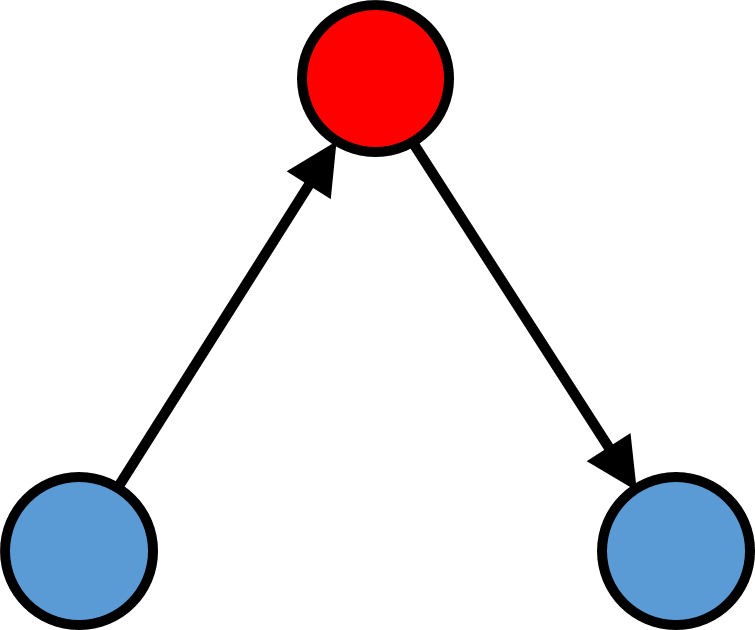
\includegraphics[width=0.4\linewidth]{Images/w_O} \end{minipage}   & \begin{tabular}[c]{l}Broker mediates contact between two\\ individuals from a single group to\\ which he or she does not belong. \end{tabular}\\ [10ex]
		w\textsubscript{I} (coordination role)		& \begin{minipage}{.2\textwidth} \centering 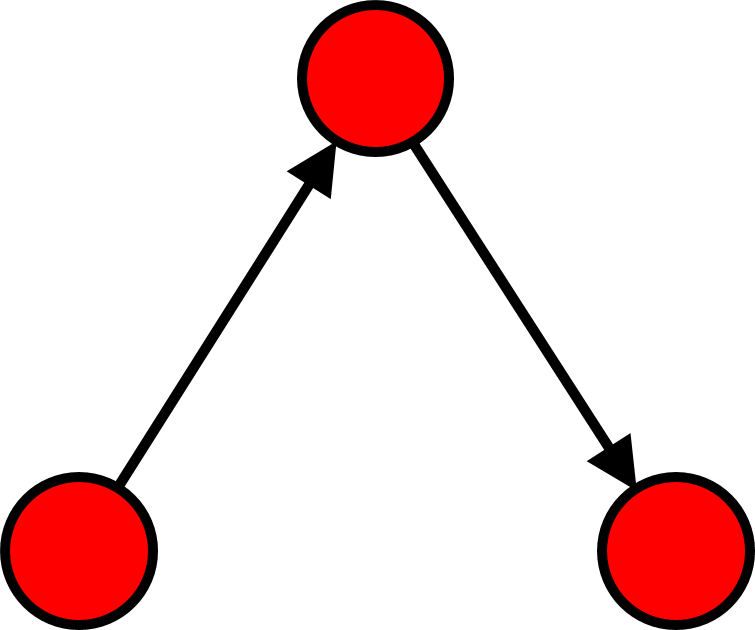
\includegraphics[width=0.4\linewidth]{Images/w_I} \end{minipage}    & \begin{tabular}[c]{l}Broker mediates contact between two\\ individuals from his or her own\\ group. \end{tabular}\\ 
		\bottomrule
	\end{tabular}
\end{table}


\citet{obstfeld2014brokerage} define brokerage more broadly as behaviour by which an actor influences, manages, or facilitates interactions between other actors.” They distinguish between brokerage emphasising a particular structural pattern (“brokerage structure”) and the social behaviour of third parties (“brokerage process”). Relaxing the central criterion for brokerage, namely the absence of ties between alters, creates a new set of cases where coordinative action by a third party might be considered \citep{obstfeld2014brokerage}. These cases are more about empowering others than empowerment of self. The social behaviour of third parties can de described in terms of conduit brokerage, tertius gaudens brokerage, and tertius iungens brokerage \citep{obstfeld2014brokerage}.\medskip

Conduit brokerage involves passing information between parties. The third party relays information from one alter to another without attempting to influence the relationship between alters. However, conduit brokerage is consistent with the knowledge advantage associated with structural holes \citep{burt1992structural}. The third-party may benefit by filtering or supplementing information passed on or expect some reward or rent in exchange for providing information \citep{obstfeld2014brokerage}. \medskip

Tertius gaudens brokerage refers to situations where a broker seeks to gain personal advantage by exploiting unfamiliarity, competition, or conflict between other parties. This may include divide and conquer tactics where the third party encourages conflict between two other parties to gain a dominating position \citep{simmel1950sociology,burt1992structural,obstfeld2014brokerage}. Passing information between parties is also central to tertius gaudens. However, the transfer of information may involve strategies where information is altered or withheld to keep alters apart or encourage conflict \citep{obstfeld2014brokerage}.\medskip

With tertius iungens brokerage, a third party introduces or facilitates interaction between two other parties. While tertius gaudens exploits disconnection or negative ties, teritius iungens actively pursues coordination. Tertius iungens brokerage is most opportune when the broker detects opportunities to connect complementary, rather than redundant, alter attributes such as resources and abilities \citep{obstfeld2014brokerage}. Both conduit and iungens draw on knowledge articulation, or the social process by which knowledge is made more explicit, useful, or relevant to the situation at hand \citep{obstfeld2005social,obstfeld2011saying,obstfeld2012creative}.\medskip

Effective brokerage strategies may require complex combinations and sequences of different brokerage behaviours over time. Skilled brokerage often involves selective deployment of these approaches with different actors or for different objectives. Different combinations of tertius iungens and tertius gaudens behavior are necessary to tailor brokerage strategies to match the situation \citep{obstfeld2014brokerage}. ... Davis’s (2011) study of innovative alliances in the computer industry found that active pruning of old ties may be necessary before man- agers can effectively facilitate new ties, suggesting that sequences of gaudens and iungens behavior are sometimes necessary.

Actors may have some kind of tie with nearly everyone in a given professional space, but might never consider collaborating unless a trusted broker functions as a tertius iungens to facilitate sufficiently increased trust to make collaboration possible. For example, trust between alters may be dependent on the presence of the broker. Alternatively, the broker facilitates the development of trust between alters, adding another dimension to their relationship \citep{obstfeld2014brokerage}.

\citet{cohen1990absorptive} see brokers with diverse expertise and contacts playing a key role in the acquisition of knowledge. They believe a diversity of internal perspectives is important to counter resistance towards external knowledge or ideas.  

\subsection{What does this mean in practice?}

, meaning that knowledge sharing acts reliably follow knowledge sharing intentions \citep{witherspoon2013antecedents}. The more benefit the individual perceives as a result of sharing knowledge, the more likely the individual is to engage in knowledge sharing \citep{bock2001breaking,witherspoon2013antecedents}.

The more internalised the individual’s motivation to share knowledge, the more likely that knowledge sharing will result \citep{gagne2009model,witherspoon2013antecedents}.

The accumulation of tacit knowledge requires considerable investment of time and resources. Those who have invested heavily in their current knowledge may not be willing to unlearn. Long-held views and knowledge acquired and reinforced over a long period of time may be considered more difficult to unlearn than recently acquired knowledge, to which the individual has less of an emotional attachment \citep{rebernik2007fostering}.

For unlearning to take place, intentional forgetting of some parts of existing individual and organizational knowledge is needed \citep{rebernik2007fostering}.

Effective knowledge management includes dealing with the defensive mechanisms that impede communication. Common defensive mechanisms include avoiding the discussion of important issues, giving ambiguous messages and distorting information. To avoid these phenomena is very important to develop a culture which values openness, tolerates failures, encourages questioning of the way things are conducted and permits workers to challenge their superiors \citep{lubit2001keys}.

